\documentclass[11pt, a4paper]{article}
%\usepackage{proj1}
\usepackage{natbib}
\usepackage{fancyhdr}  
\usepackage{subcaption}
\usepackage{caption}
\usepackage{graphicx}
\usepackage{numprint}
\usepackage{multirow}
\linespread{1.25} 
\setlength{\parindent}{0cm}
\graphicspath{{Images/}}
\usepackage{hyperref}
\usepackage{amsmath}
\usepackage{amsfonts}
\usepackage{amssymb}
\usepackage{amsthm}
\usepackage{mathtools}
\usepackage{commath}
\usepackage{bbm}

%\usepackage[sc,osf]{mathpazo}
\usepackage{subcaption}
\usepackage[a4paper, top=1in, left=1.0in, right=1.0in, bottom=1in, includehead, includefoot]{geometry} %Usually have top as 1in

\usepackage{listings}
\usepackage{color} %red, green, blue, yellow, cyan, magenta, black, white
\definecolor{mygreen}{RGB}{28,172,0} % color values Red, Green, Blue
\definecolor{mylilas}{RGB}{170,55,241}


\hypersetup{colorlinks,linkcolor={black},citecolor={blue},urlcolor={black}}
\usepackage{color}
\urlstyle{same}


\theoremstyle{definition}
\newtheorem{definition}{Definition}[section]

%\newcommand{\Sta}{\rho}
\newcommand{\Adj}{p}
\newcommand{\adj}{q}
%\newcommand{\Con}{u}
\newcommand{\Sta}{\rho}
\newcommand{\Stav}{\mathbf{v}}
\newcommand{\Adja}{\mathbf{p}}
\newcommand{\Adjb}{q}
\newcommand{\Adjc}{{p}_{\partial \Sigma}}
\newcommand{\Con}{\mathbf{f}}
\newcommand{\nor}{\mathbf{n}}




\pagenumbering{gobble}
\begin{document}
	\section{Report 10/09/2020}

	
	
	\section{Sparse to Fine}
	Running a problem on a sparse grid and interpolating onto a fine one. The sparse grid is $N = n = 10$, the fine one is $N = 20$, $n = 10$. The tolerances for the sparse grid are $0.1/10^{-4}$ and for the fine grid they are $10^{-3}/10^{-7}$. The sparse grid problem converges in $118$ iterations, and takes $57$ seconds (around $0.5$ s per iteration). The fine grid however converges in $669$ iterations and $6.2888 \times  10^3$ seconds (around $9$ s per iteration). So there is no gain in doing this; at least not the way I have implemented this. I only tested one example though, so there may be a case for looking into this more.
	
	\section{In and outflow problem}
	Something weird is going on with this problem. I set up a target which has a small inflow, so that mass accumulates at the outflow, see Figure \ref{F01}. Then I set the OCP so that the in and outflows are both $1$ and $\rho$ is also $1$ initially. I would expect it wants to force mass to the outflow. Instead it accumulates mass at the inflow. This happens for other targets too.
	See Figure \ref{F02} and \ref{F03} for the first iteration solution. After two iterations, $\rho$ gets pushed up that boundary to $200$, which I think is what causes this to crash.
	\begin{figure}[h]
		\centering
		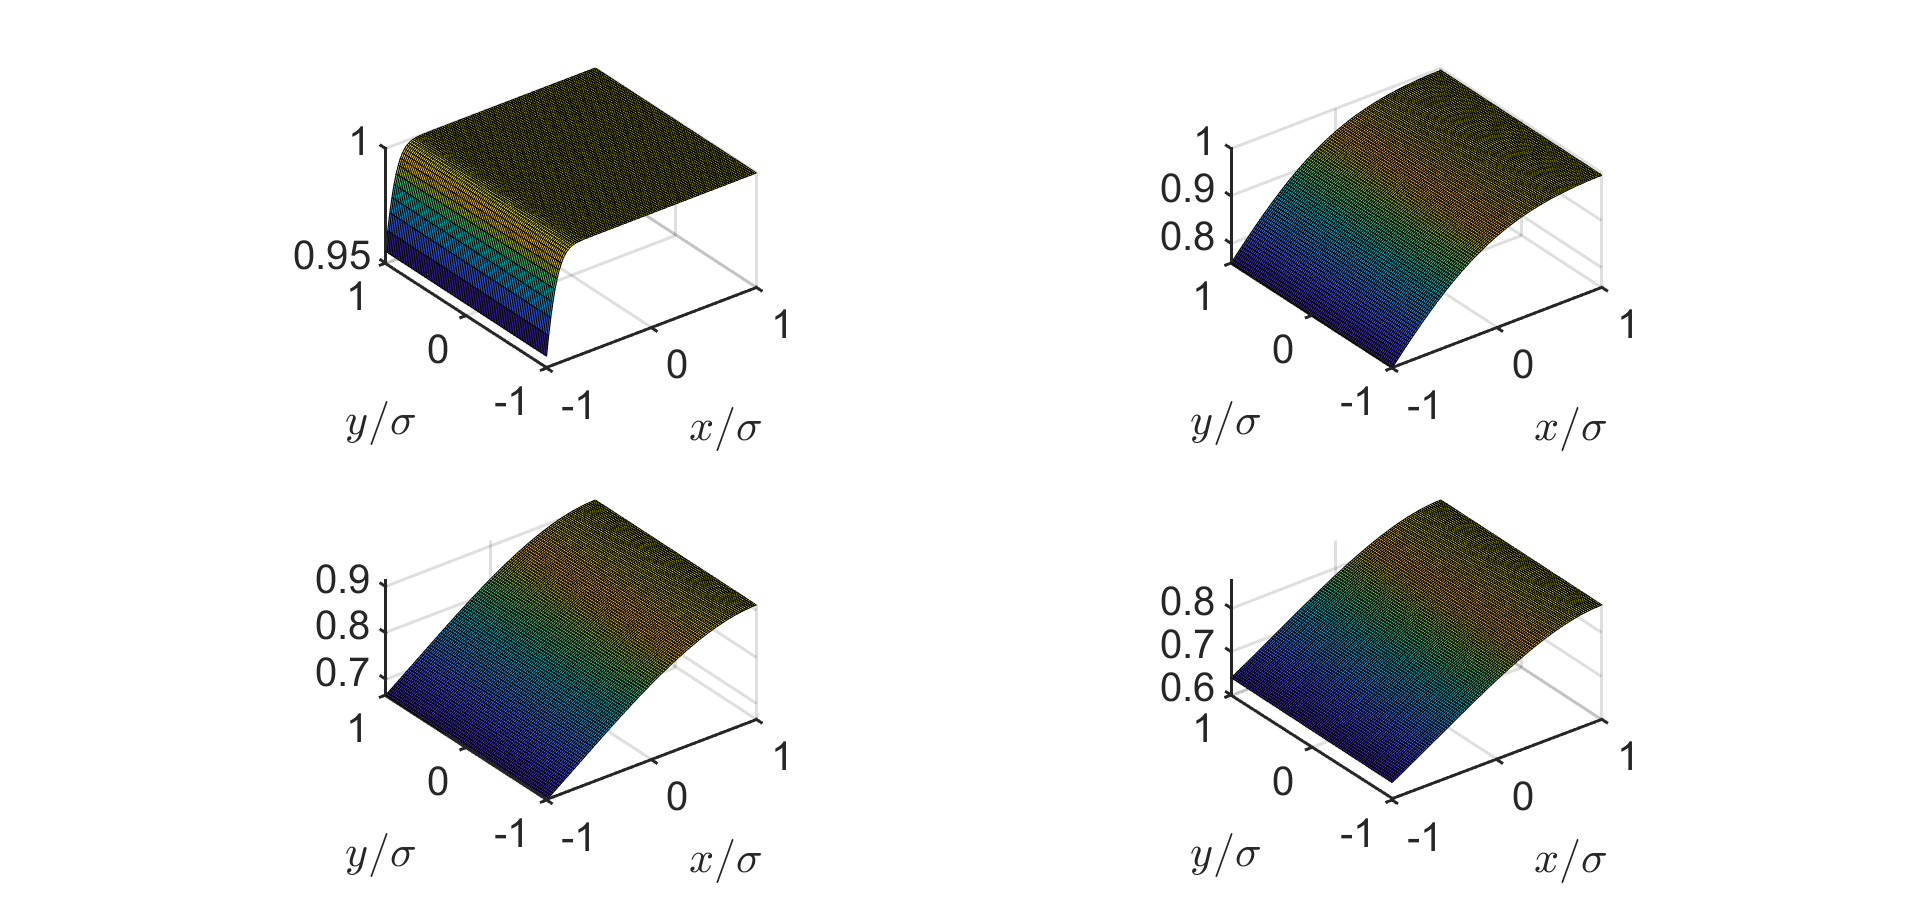
\includegraphics[scale=0.4]{InOutFW.png}
		\caption{Target} 
		\label{F01}
	\end{figure}
	\begin{figure}[h]
	\centering
	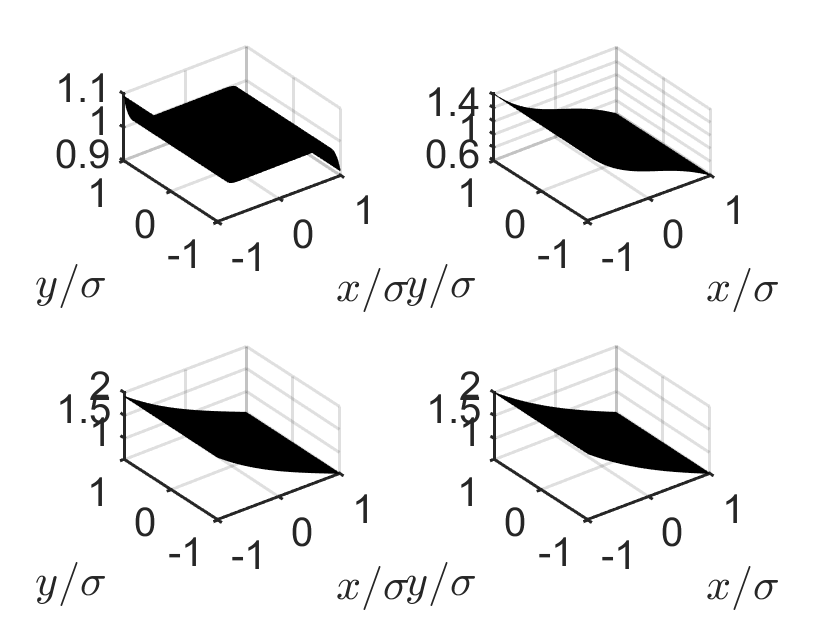
\includegraphics[scale=0.6]{InOutRho.png}
	\caption{$\rho$ after one iteration} 
	\label{F02}
    \end{figure}
	\begin{figure}[h]
	\centering
	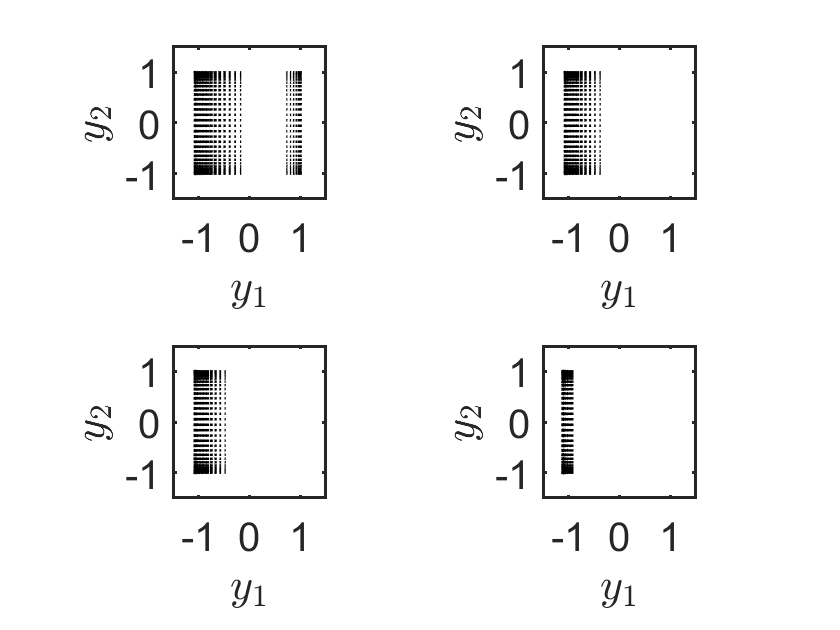
\includegraphics[scale=0.6]{InOutFlow.png}
	\caption{$\vec w$ after one iteration} 
	\label{F03}
    \end{figure}
	
	\section{Interpolation Issue}
	The issue was that some points got lost in the interpolation matrix. Figure \ref{FPts} shows where they got lost. This indicates that they are too close together and get deleted at a later point. This is fixed by adding a small value to the boundaries of the shape, see Figure \ref{FBound}. Is that allowed/ okay to do. It seems to fix the problem anyway.
		\begin{figure}[h]
		\centering
		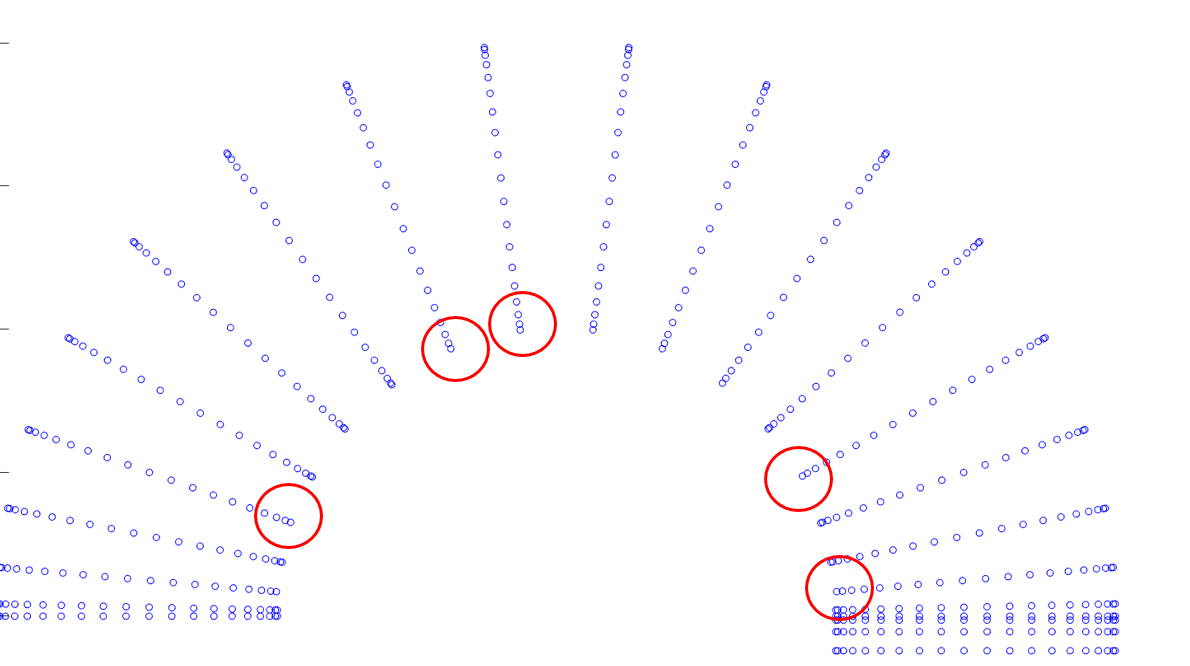
\includegraphics[scale=0.6]{Screenshot1.png}
		\caption{Missing points} 
		\label{FPts}
	\end{figure}
	\begin{figure}[h]
		\centering
		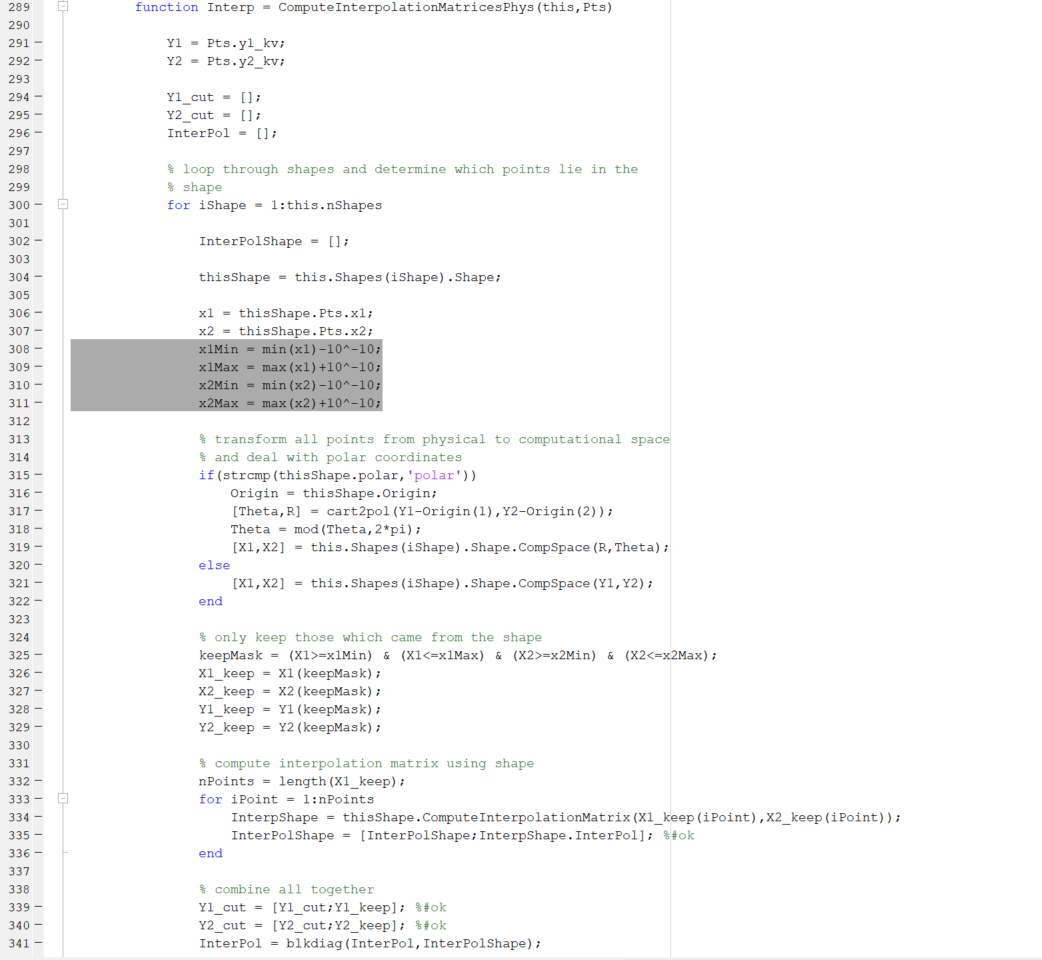
\includegraphics[scale=0.6]{InterpolatePhys.png}
		\caption{Interpolation Code} 
		\label{FBound}
	\end{figure}
	
	\section{Examples}
	\subsection{Adaptive $\lambda$}
	We use an adaptive $\lambda$ for the below examples to decrease computational time. We do this as follows:\\
	Set $k = 0$ and $k$ increases by one per iteration.
	\begin{enumerate}
		\item If $\mathcal{E}_n$ > $\mathcal{E}_o$, and $k > 10$, set $k = k -10$, and $w_{i+1} = w_i$.
		\item Elseif $\mathcal{E}_n$ > $\mathcal{E}_o$, and $k < 10$, set $k = k$, and $w_{i+1} = w_i$.
		\item If $\mathcal{E}_n$ = $\mathcal{E}_o$, the $\lambda = 0.5\lambda$, and $w_{i+1}$ is found by mixing scheme.
		\item If $\mathcal{E}_n$ < $\mathcal{E}_o$, them:
		\begin{itemize}
			\item if $k < 10$, $\lambda = 0.01$.
			\item if $k < 20$, $\lambda = 0.02$.
			\item if $k < 30$, $\lambda = 0.03$.
			\item if $k < 40$, $\lambda = 0.05$.
			\item if $k < 50$, $\lambda = 0.06$.
			\item if $k < 60$, $\lambda = 0.08$.
			\item else, $\lambda = 0.1$.
		\end{itemize}
	\end{enumerate}
After running the examples, I now changed step 2 to be the same as step 3.
	\subsection{Example1}
	Note: for $T = 1$, we had each iteration at $80$ seconds. Now it is $35$ seconds. Also. We had convergence in $500 -600$ iterations. Now it is around $100$.\\
	\\
	This example runs with $T = 1.75$. We choose $N = n = 20$, tols $ 10^{-7}/ 10^{-3}$ and $\beta = 10^{-3}$.
	For $\kappa = -1$ we get convergence in $125$ iterations, which takes $4.4314 \times 10^3$ seconds, which is around $ $ seconds per iteration. $J_{FW} = 0.3654$, $J_{Opt} = 0.0661$. See Figures \ref{F1} and \ref{F2}.
	\begin{figure}[h]
		\centering
		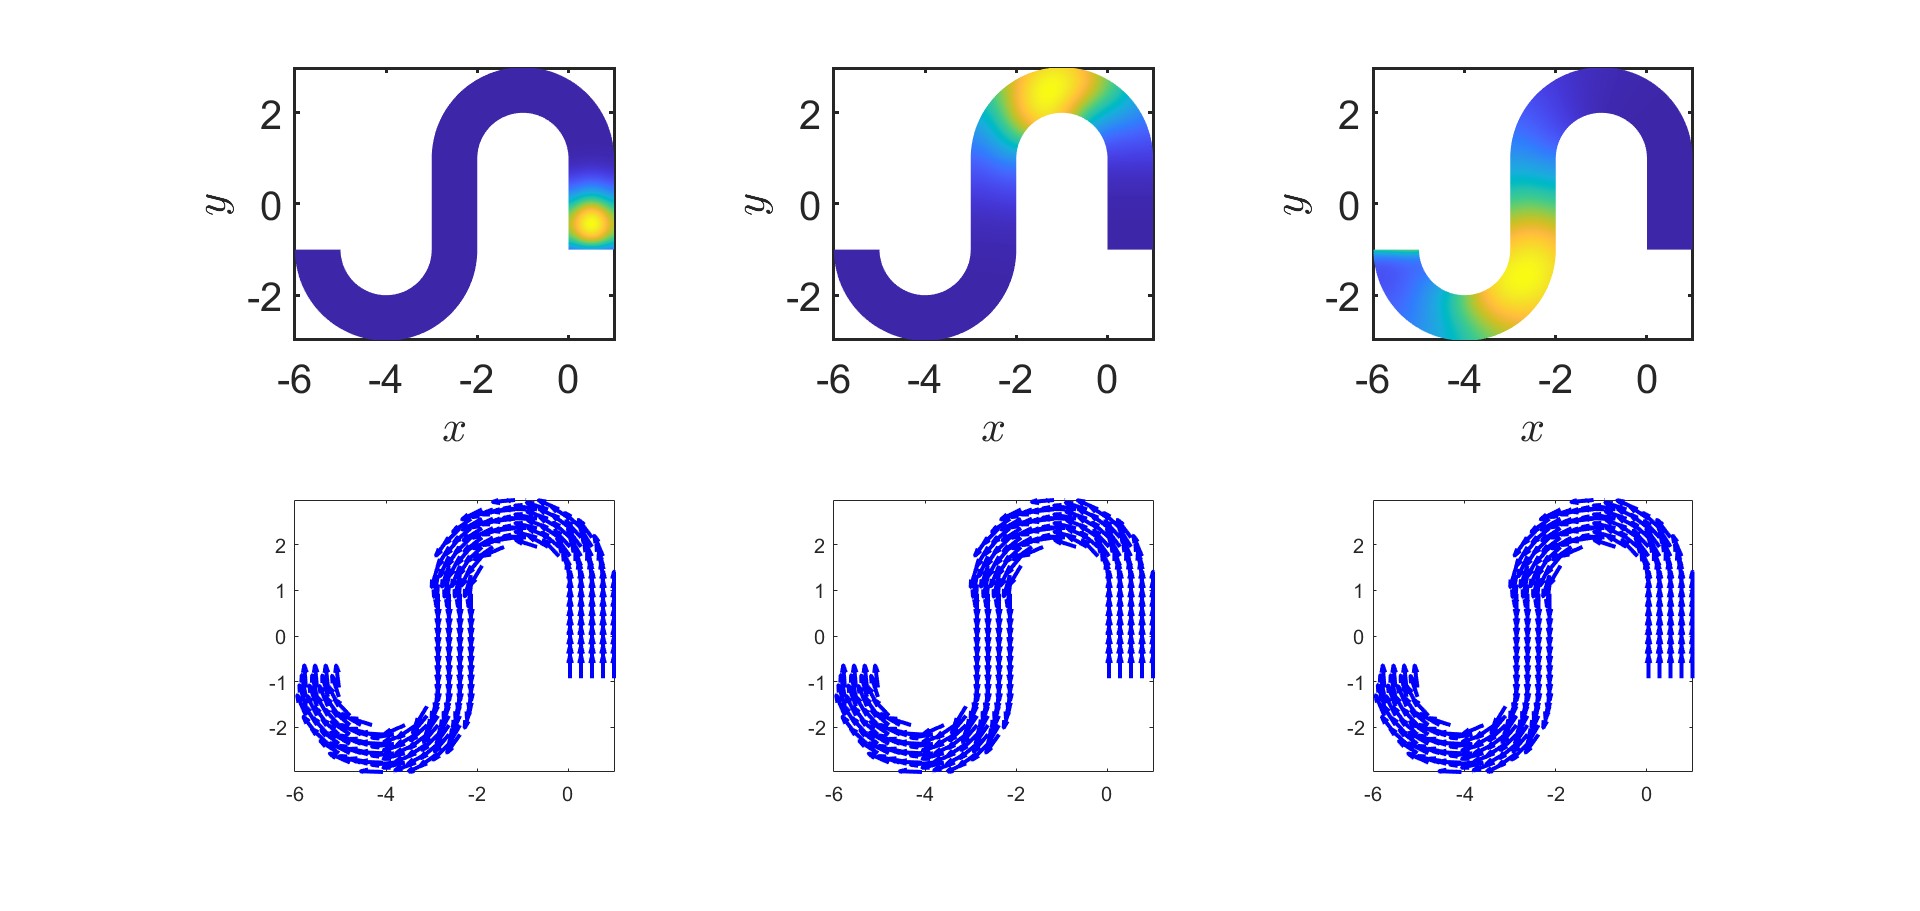
\includegraphics[scale=0.35]{FW11kn1.png}
		\caption{Target with $\kappa = -1$} 
		\label{F1}
	\end{figure}
	\begin{figure}[h]
		\centering
		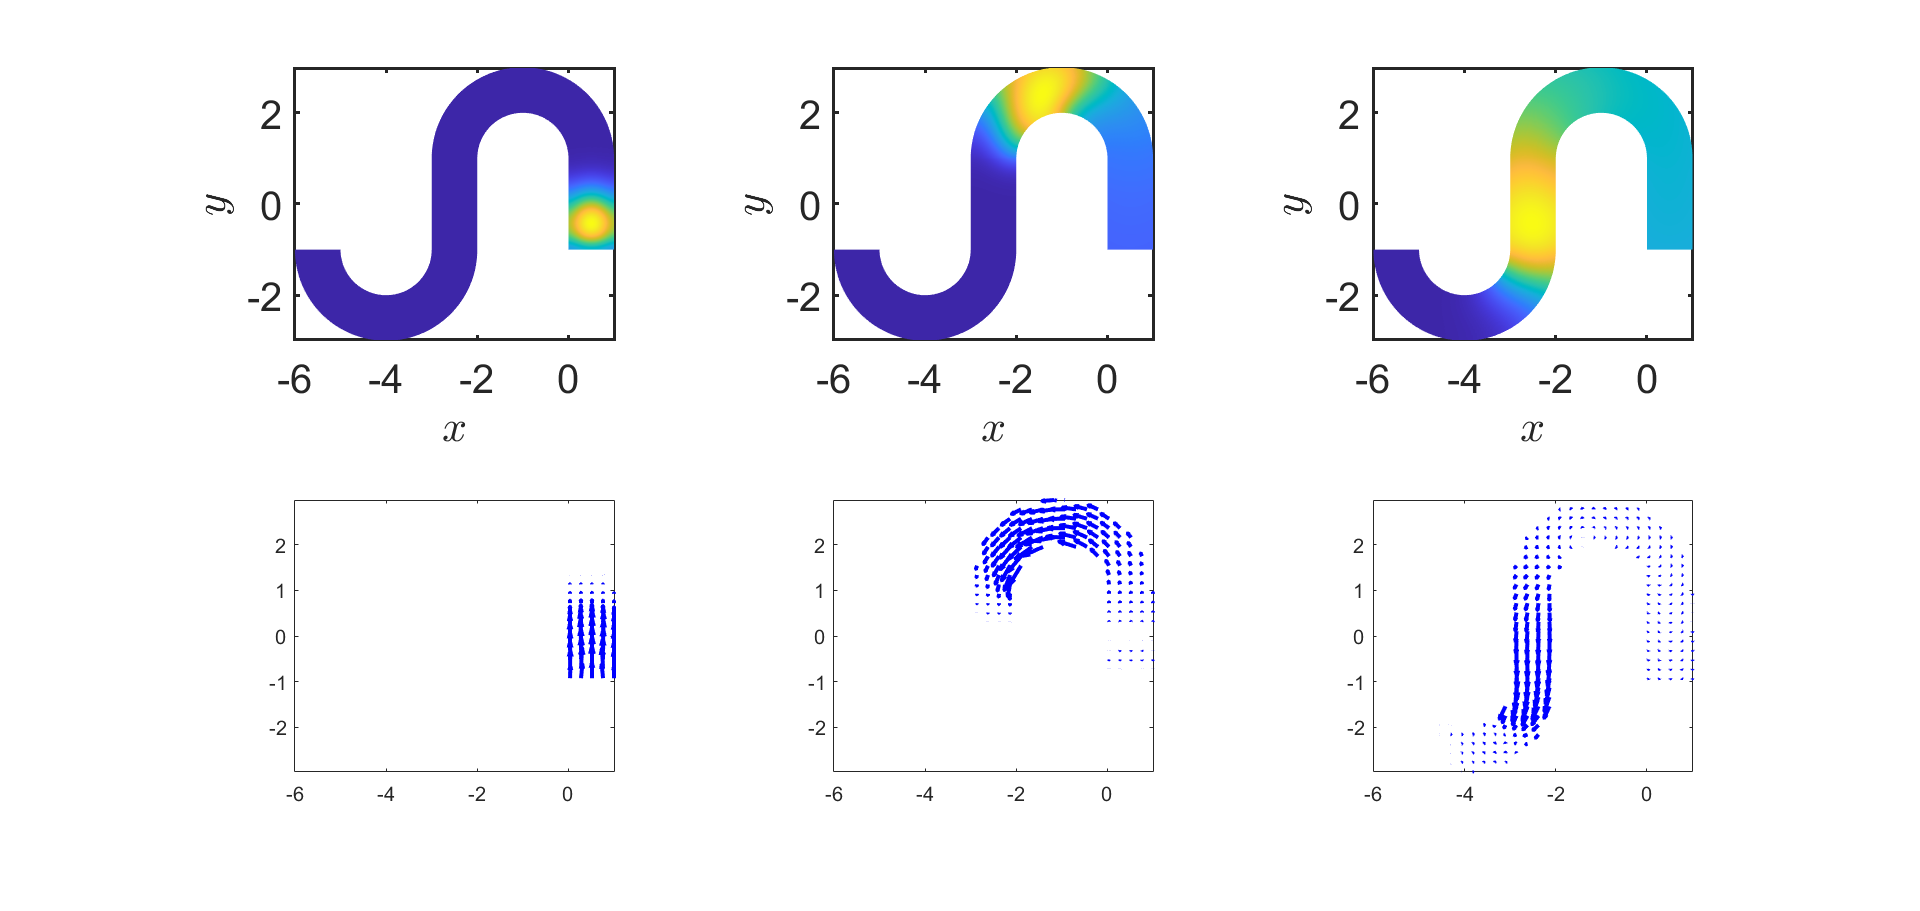
\includegraphics[scale=0.35]{Opt11kn1.png}
		\caption{Optimal Result with $\kappa = -1$} 
		\label{F2}
	\end{figure}
	For $\kappa = 1$ we get convergence in $114$ iterations, which takes $4.0090 \times 10^3$ seconds, which is around $35$ seconds per iteration. $J_{FW} = 0.3090$, $J_{Opt} = 0.0667$.See Figures \ref{F3} and \ref{F4}.
	\begin{figure}[h]
		\centering
		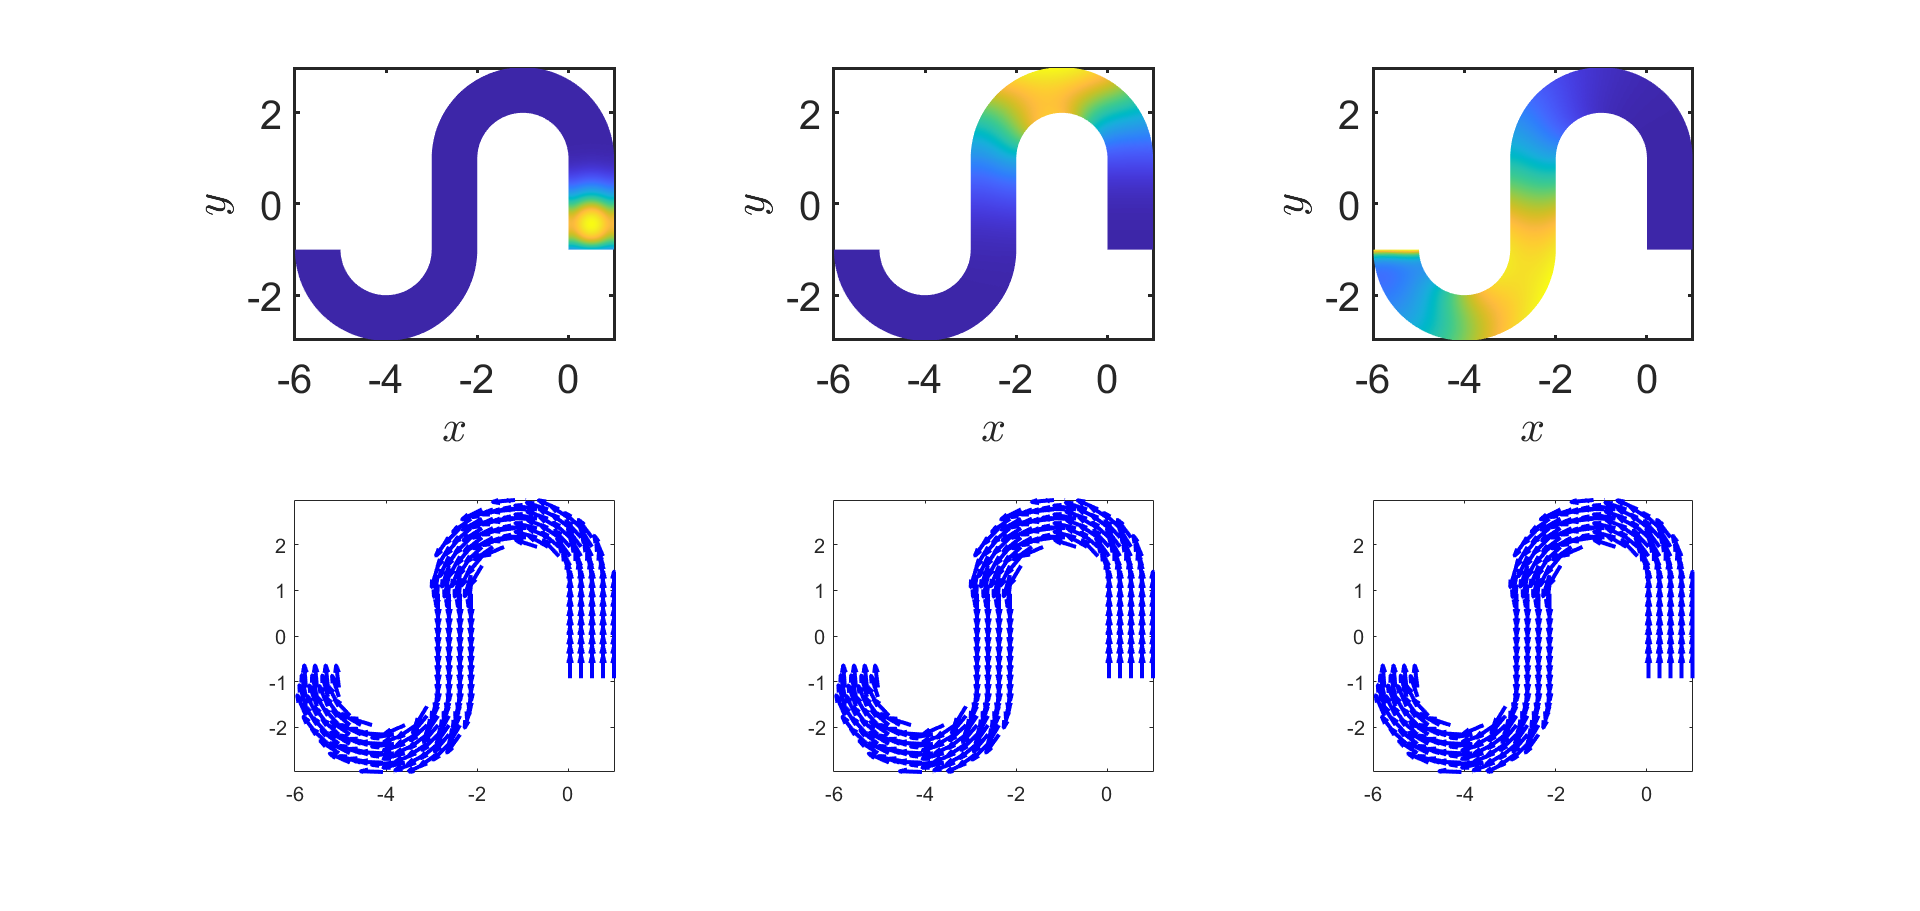
\includegraphics[scale=0.35]{FW11k1.png}
		\caption{Target with $\kappa = 1$} 
		\label{F3}
	\end{figure}

	\begin{figure}[h]
		\centering
		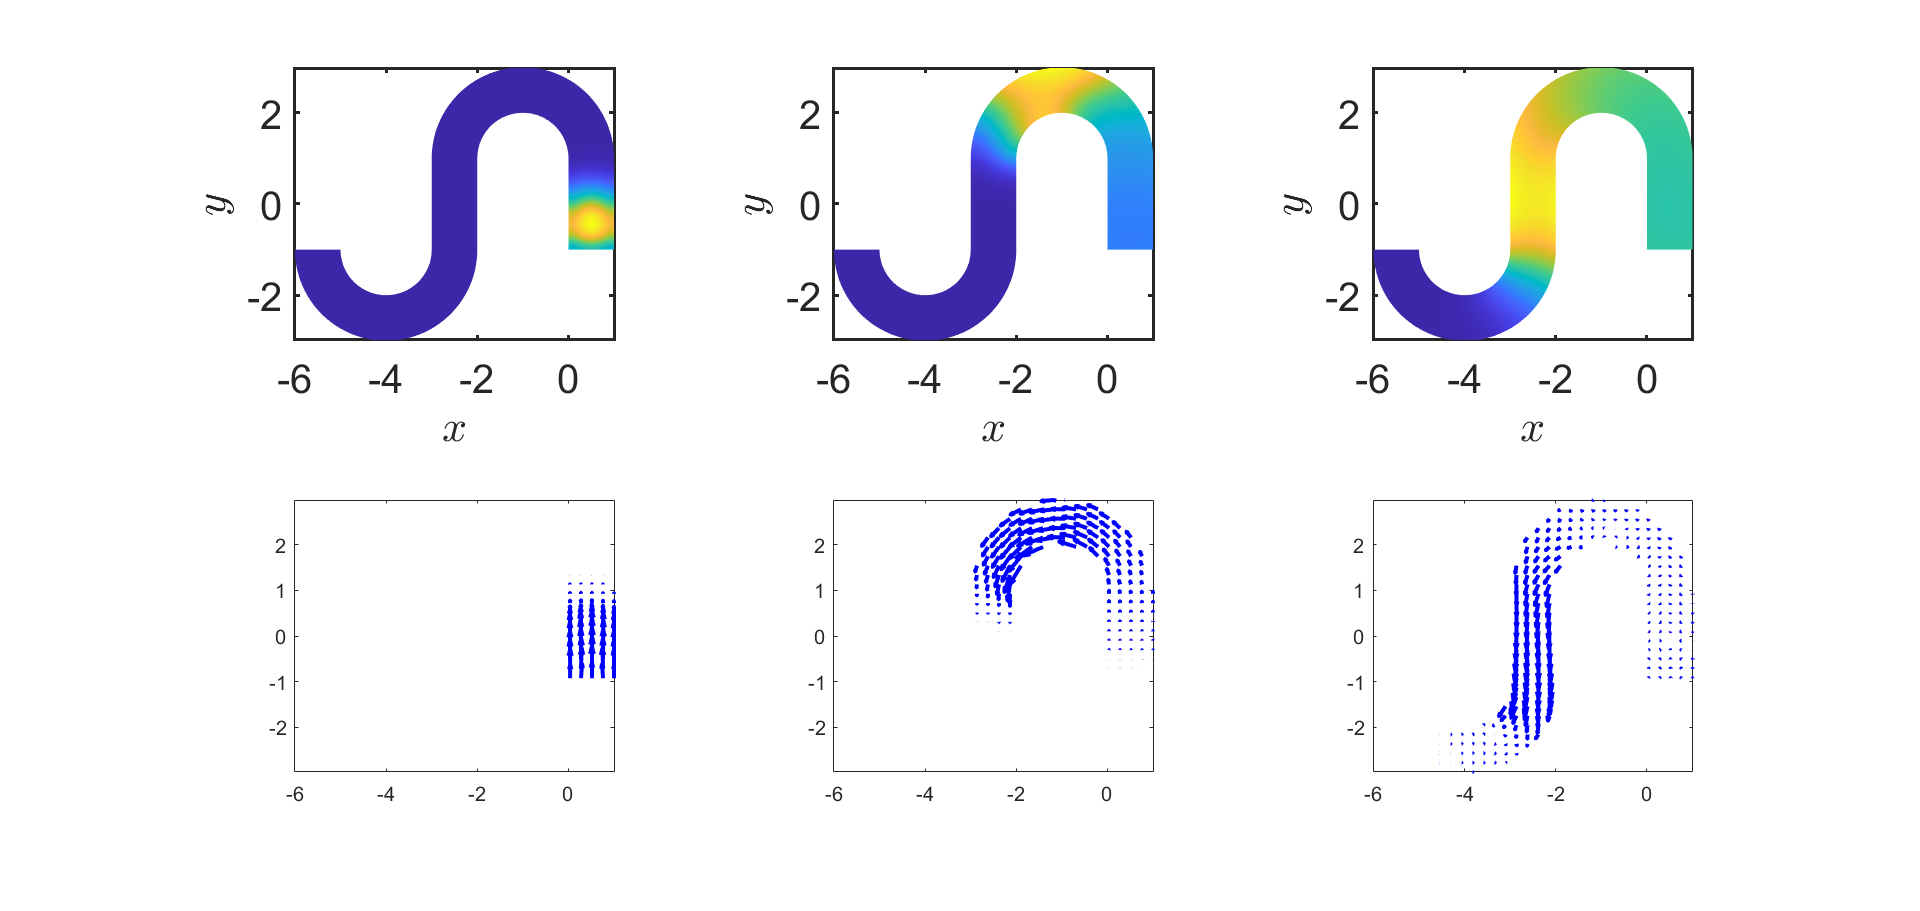
\includegraphics[scale=0.35]{Opt11k1.png}
		\caption{Optimal Result with $\kappa = 1$} 
		\label{F4}
	\end{figure}

In both examples, in the OCP, the flow does not match the one from the target at the end. I think this is due to $\vec w = \vec = 0$ at $T$.
\subsection{Example 2}
	This is adapted from the original 'fancy channel'. Running the original takes a lot longer because there are more shapes involved. \\
	In comparison: without the fix for time this would take $32$ seconds per iteration (around $20$ now). Without the Adaptive algorithm, it would take $467$ iterations (around $100$ now) to solve the problem with $\kappa = 0$. See Figures \ref{F9} and \ref{F10}.
    \begin{figure}[h]
		\centering
		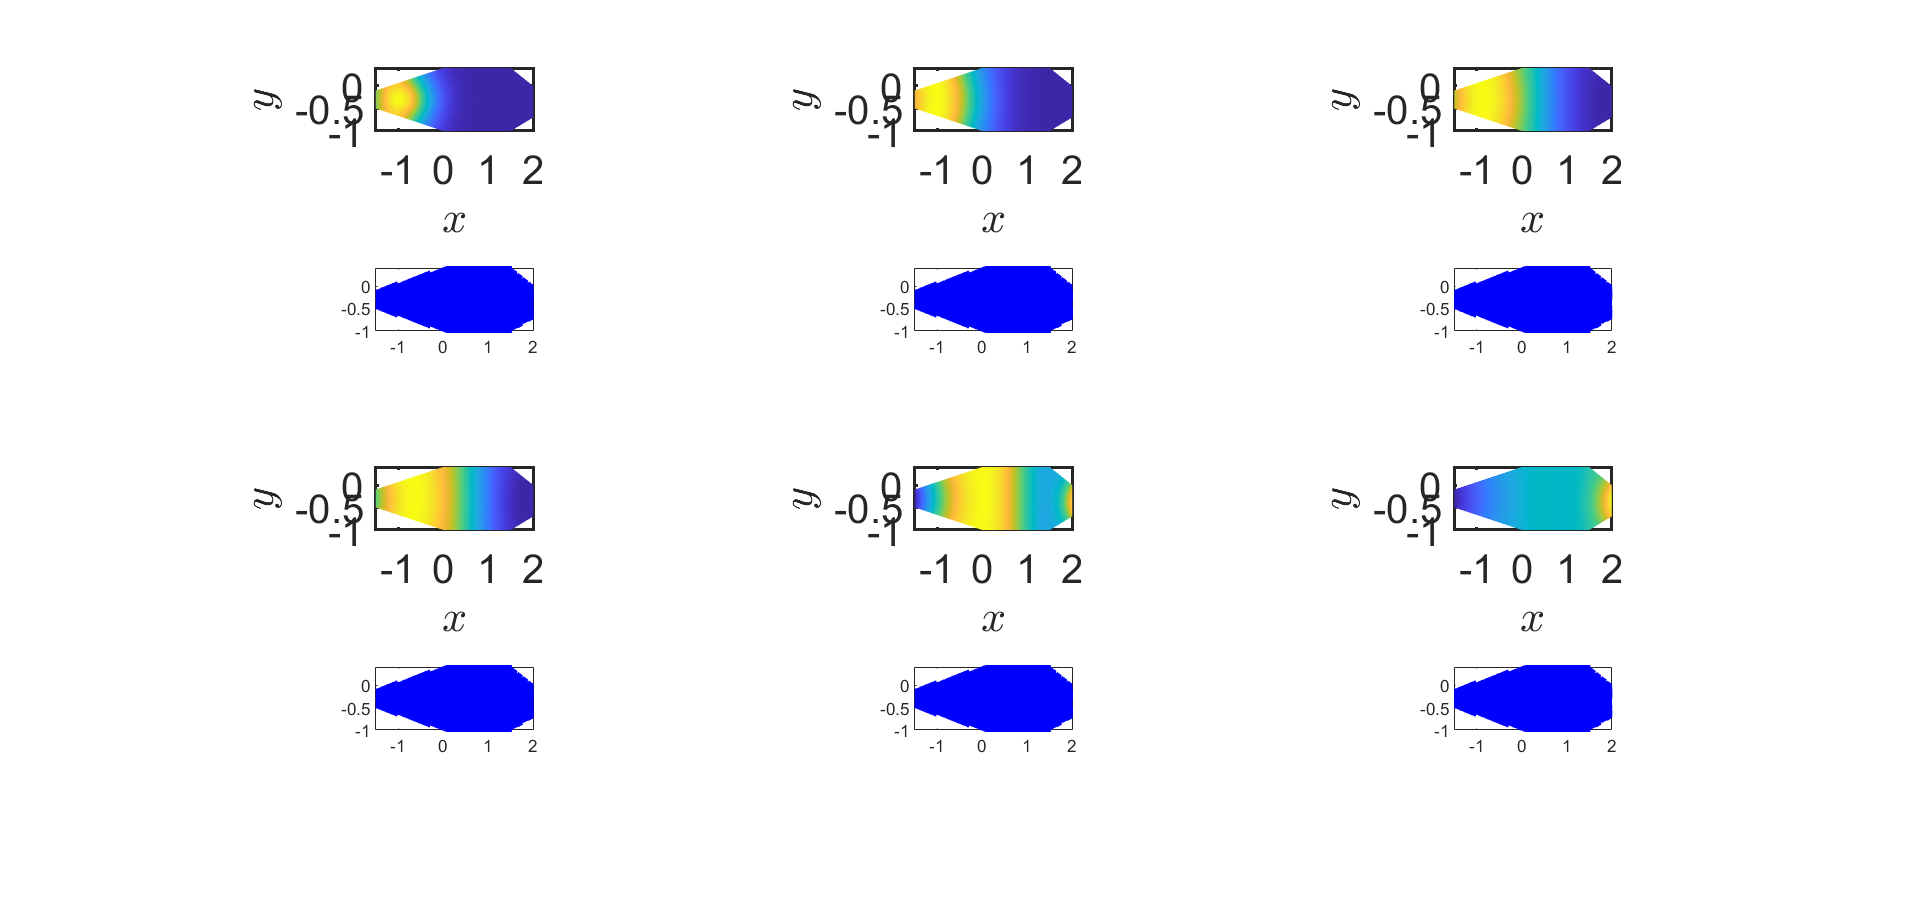
\includegraphics[scale=0.35]{FWChannelk0.png}
		\caption{Forward Problem with $\kappa = 0$} 
		\label{F9}
	\end{figure}
	
	\begin{figure}[h]
		\centering
		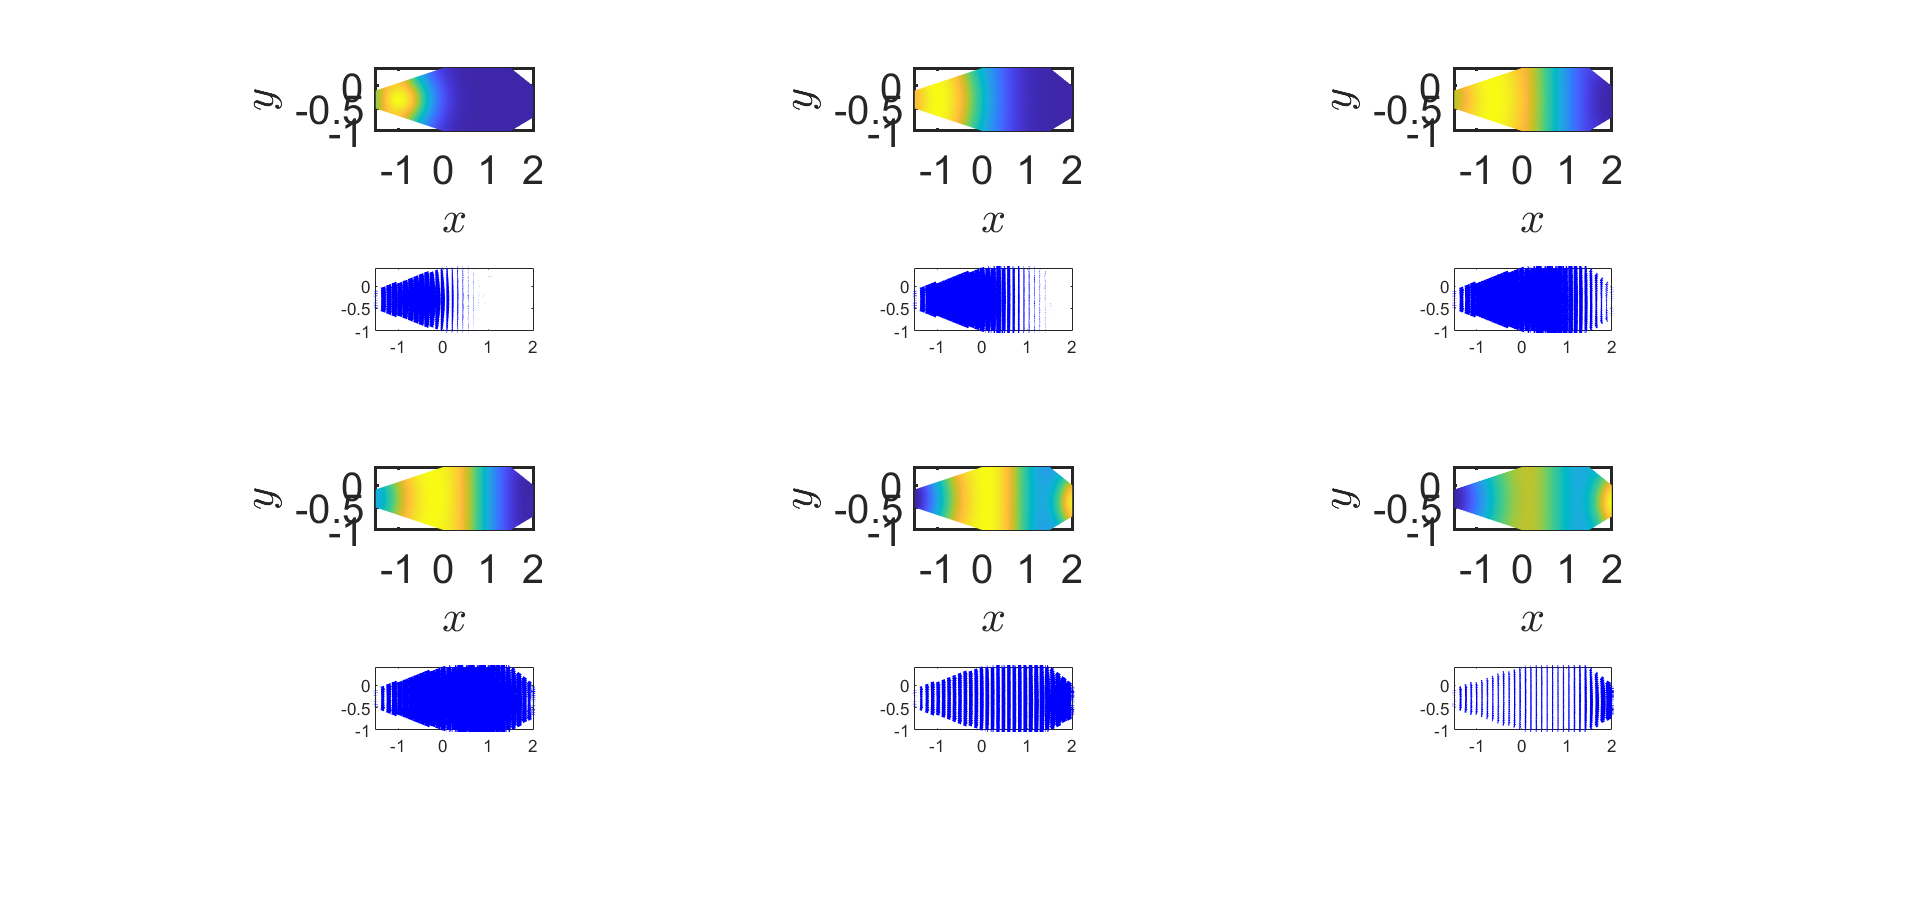
\includegraphics[scale=0.35]{OptChannelk0.png}
		\caption{Optimal Result with $\kappa = 0$} 
		\label{F10}
	\end{figure}
	For $\kappa = -1$ we get convergence in $101$ iterations, which takes $1.9365 \times 10^3$ seconds, which is around $20$ seconds per iteration. $J_{FW} = 0.0184$, $J_{Opt} = 9.5323 \times 10^{-4}$. See Figures \ref{F5} and \ref{F6}.
	\begin{figure}[h]
		\centering
		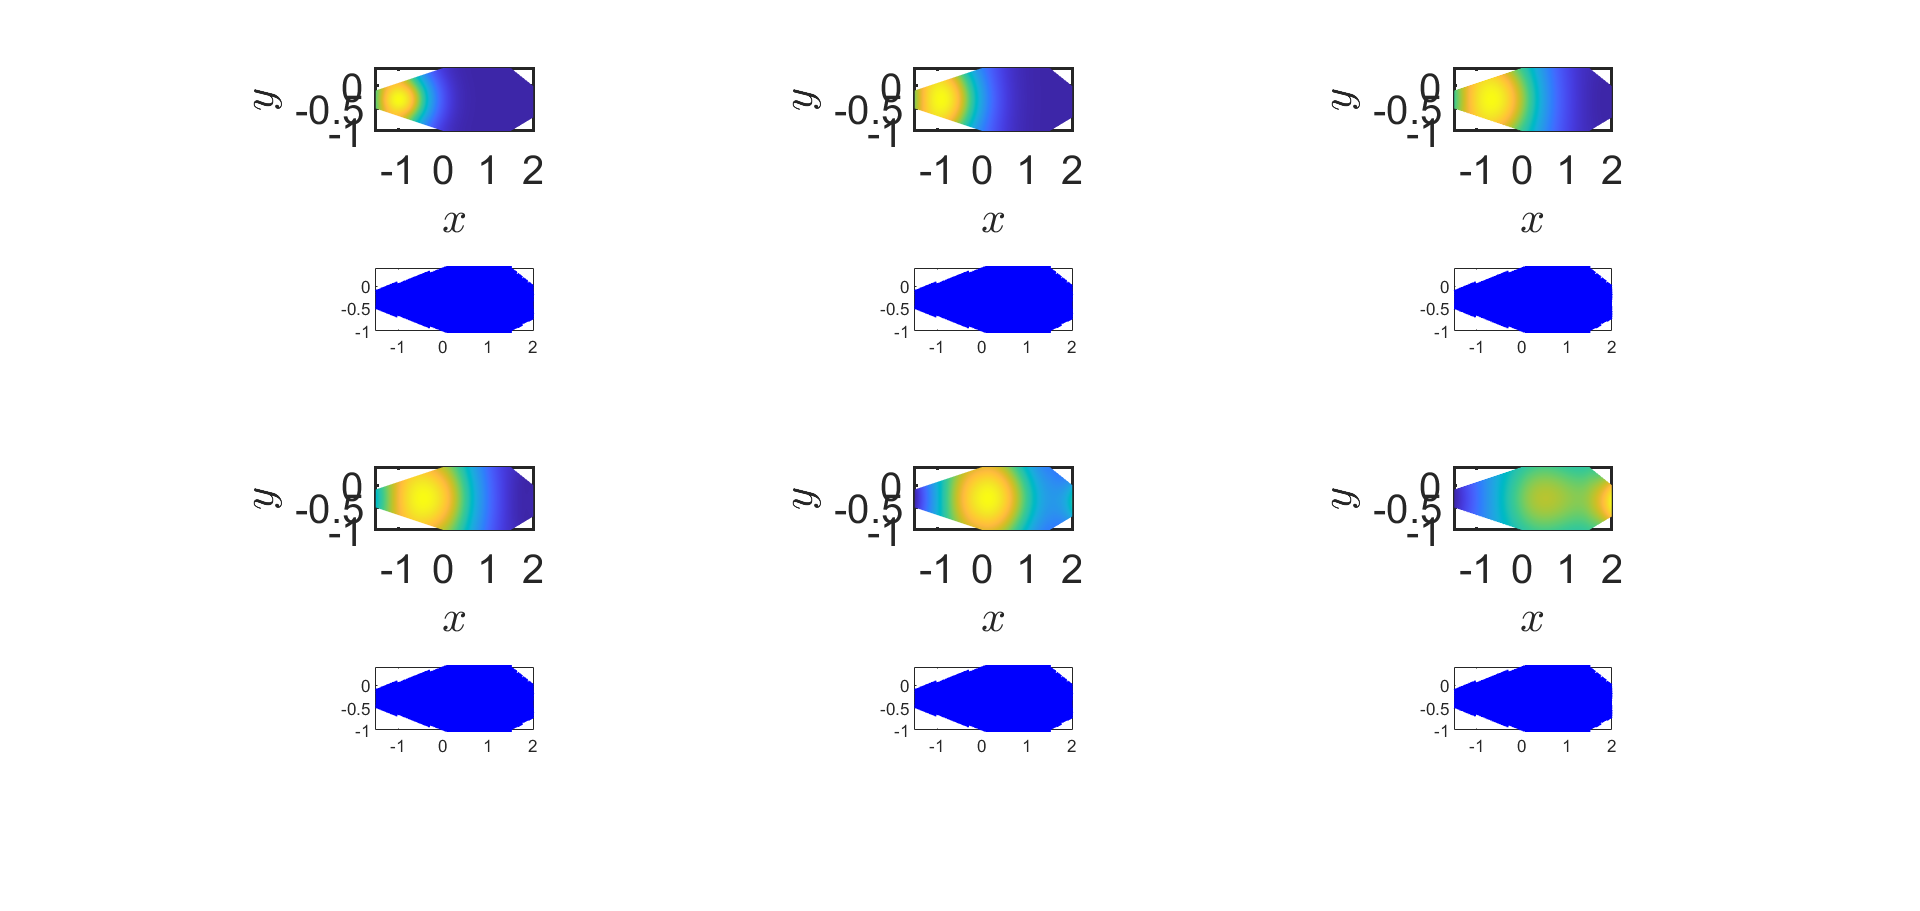
\includegraphics[scale=0.35]{FWChannelkn1.png}
		\caption{Forward Problem with $\kappa = -1$} 
		\label{F5}
	\end{figure}
	
	\begin{figure}[h]
		\centering
		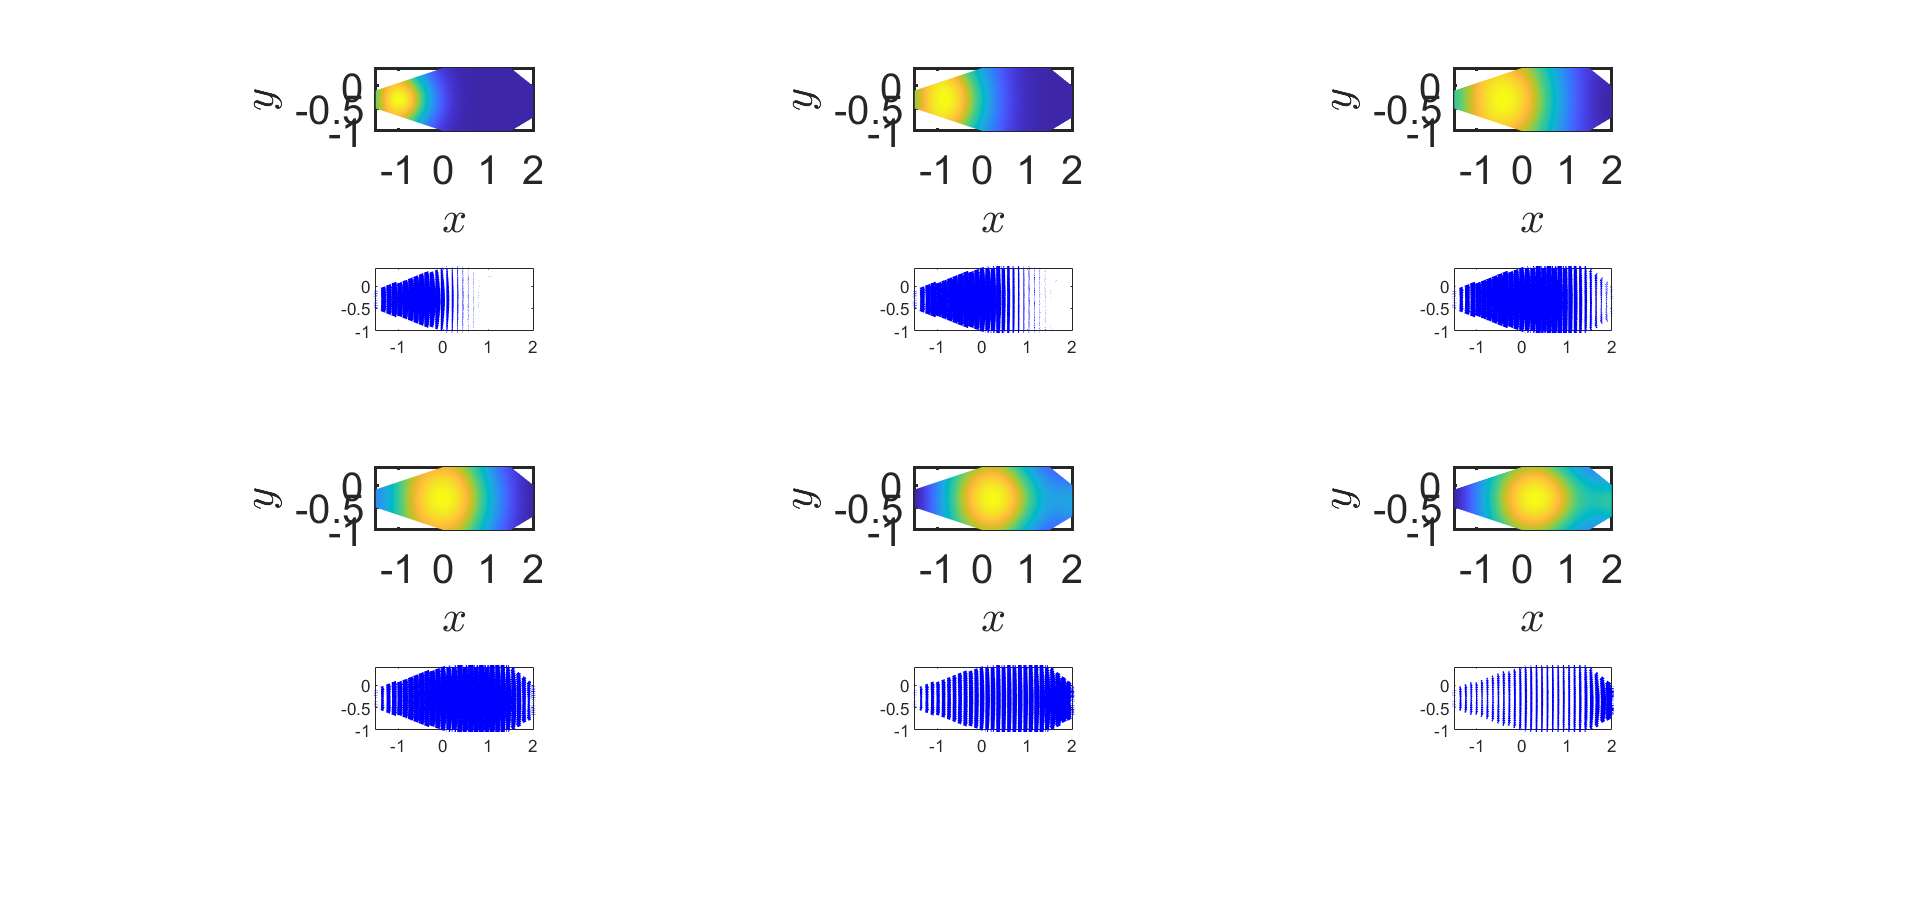
\includegraphics[scale=0.35]{OptChannelkn1.png}
		\caption{Optimal Result with $\kappa = -1$} 
		\label{F6}
	\end{figure}
	For $\kappa = 1$ we get convergence in $87$ iterations, which takes $1.6845 \times 10^3$ seconds, which is around $20$ seconds per iteration. $J_{FW} = 0.0150$, $J_{Opt} = 0.0010$. See Figures \ref{F7} and \ref{F8}.
		
	
	\begin{figure}[h]
		\centering
		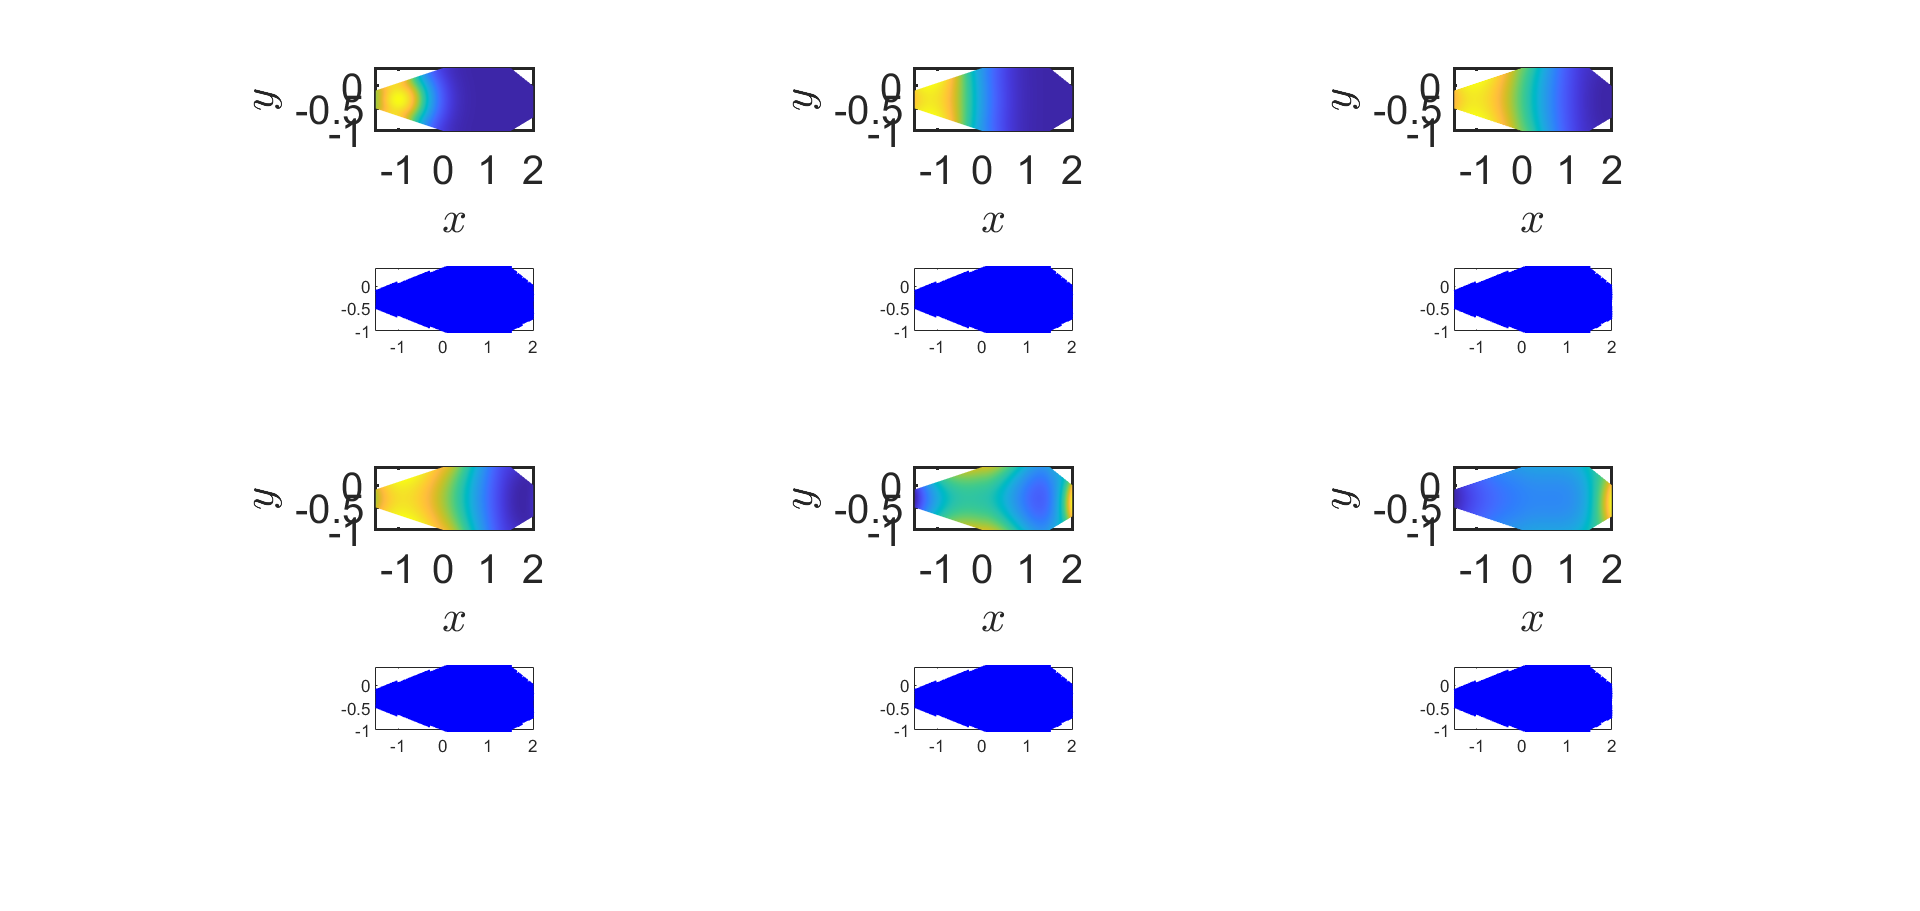
\includegraphics[scale=0.35]{FWChannelk1.png}
		\caption{Forward Problem with $\kappa = 1$} 
		\label{F7}
	\end{figure}
	
	\begin{figure}[h]
		\centering
		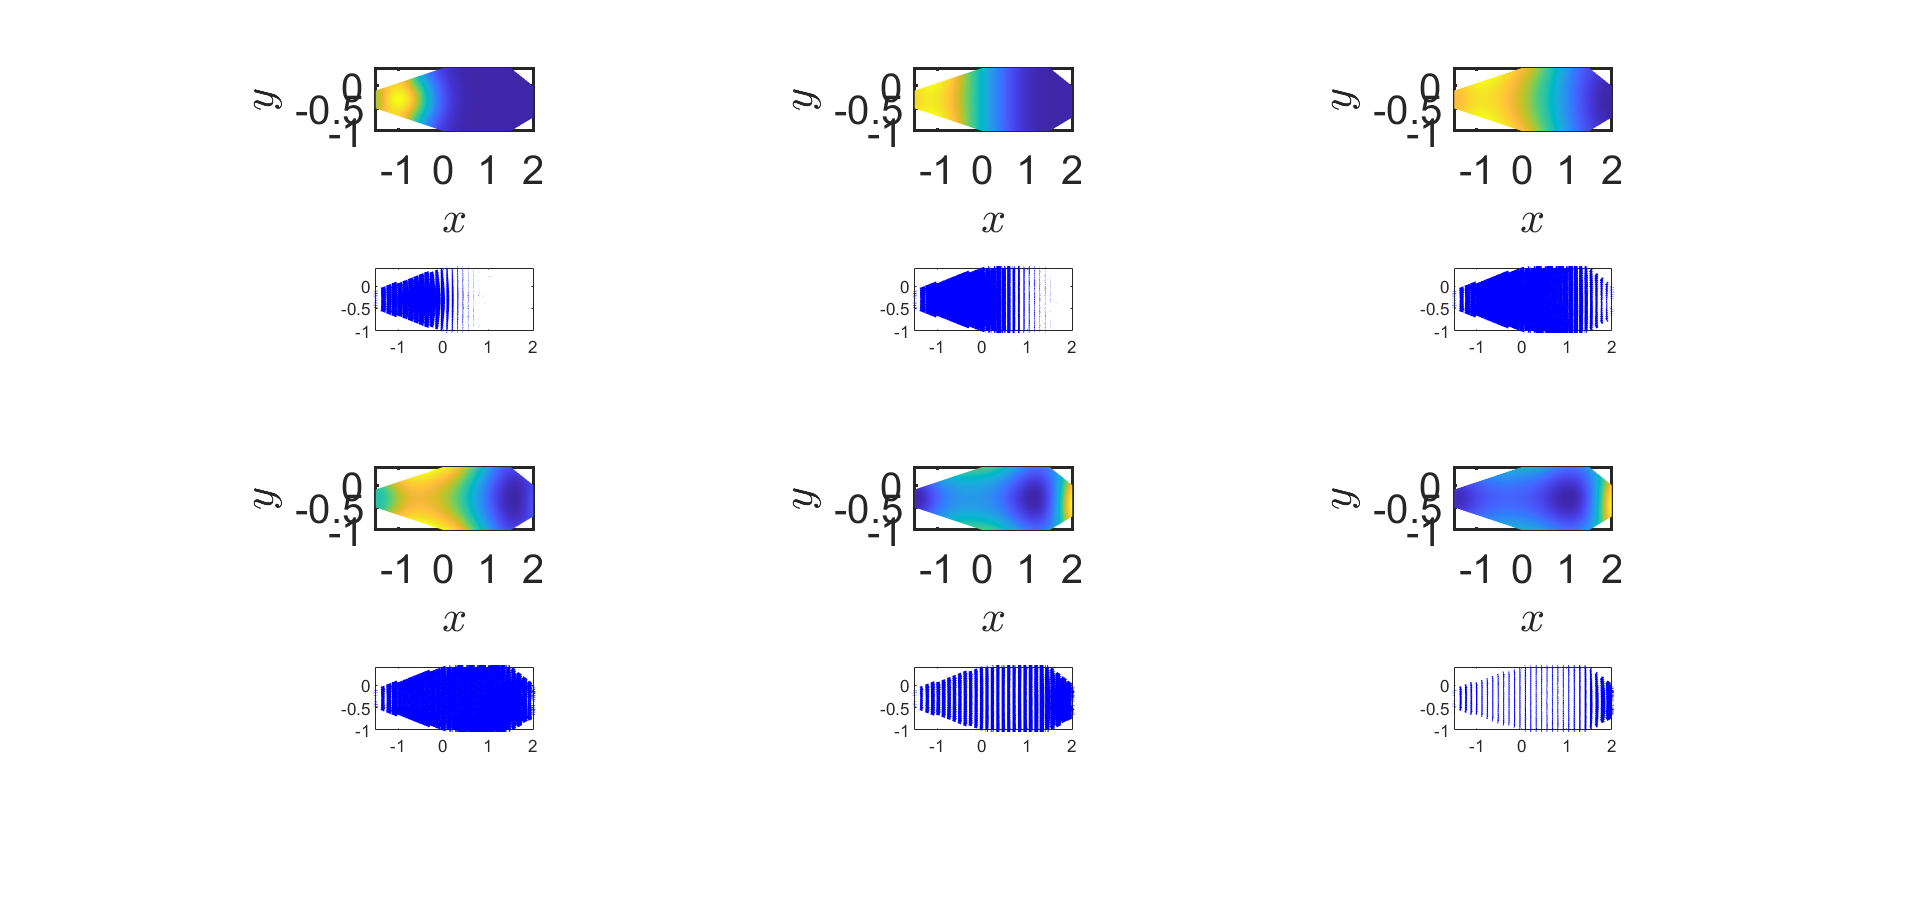
\includegraphics[scale=0.35]{OptChannelk1.png}
		\caption{Optimal Result with $\kappa = 1$} 
		\label{F8}
	\end{figure}

\section{Other}
- Memory issue with datastorage.
\\
\\
- Background section: Some DDFT background and some statistical mechanics stuff?\\
\\
- Classes: As discussed last week, it makes most sense to take the MAC-MIGS course for credit this semester and the Python course for general skills credits. I am enrolled in Fundamentals of Optimization as class only student.\\
If possible, I would like to be enrolled in the following School of Informatics courses:
'Design and Analysis of Parallel Algorithms' and 'Numerical Algorithms for High Performance Computing'. 
I am not sure if these are what I think they are, but I would just like to have a look.
	
\end{document}